\documentclass[11pt,a4paper]{article}

\usepackage[top=1.7cm,bottom=1.9cm,left=1.9cm,right=1.9cm]{geometry}
\usepackage{amsmath,amssymb}
\usepackage{booktabs}
\usepackage{graphicx}
\usepackage{caption}
\usepackage{subcaption}
\usepackage[hidelinks]{hyperref}
\usepackage{parskip}
\usepackage{titlesec}
\usepackage{placeins}
\usepackage{float}

\titleformat{\section}{\normalfont\large\bfseries}{\thesection}{0.6em}{}
\titleformat{\subsection}{\normalfont\normalsize\bfseries}{\thesubsection}{0.5em}{}
\titlespacing{\section}{0pt}{0.4em}{0.1em}
\titlespacing{\subsection}{0pt}{0.3em}{0.05em}

\setlength{\parskip}{2pt}
\setlength{\parindent}{0pt}

\title{\vspace{-2.5em}SF2943 Project --- Part A\\[1pt]
\large Daily electricity load for Swedish bidding zone SE\_3}
\author{}
\date{}

\begin{document}
\maketitle
\vspace{-3.6em}

\section{Data}
We model daily mean electricity load (MW) for the Swedish bidding zone
\textbf{SE\_3} (Stockholm, M\"alardalen, eastern Sweden), sourced from
\emph{Open Power System Data} (OPSD), \texttt{time\_series\_60min\_singleindex.csv},
column \texttt{SE\_3\_load\_actual\_entsoe\_transparency} (originally ENTSO-E
Transparency Platform).\footnote{\url{https://data.open-power-system-data.org/time_series/}}
The hourly file covers 2015-01-01\,01:00 to 2020-09-30\,22:00 UTC
(50\,398 hourly observations, 77 NaN, longest gap 49~h). We aggregate to daily
means (units preserved); days with fewer than 20 valid hours are marked NaN
and the remaining 5 NaN days are linearly interpolated, giving
$n = 2100$ daily observations $X_t$, well above the $N \geq 2000$ threshold.

\section{Cleaning to stationarity}
Raw $X_t$ has a winter peak / summer trough cycle, a weekday/weekend cycle, a
mild secular trend and an amplitude that grows with the level. We use the
classical decomposition (B\&D~\S1.5) on the log-transformed series:
\begin{equation}
\log X_t \;=\; m_t \;+\; s_t^{(\mathrm{year})} \;+\; s_t^{(\mathrm{week})} \;+\; Y_t,
\label{eq:decomp}
\end{equation}
fitted in the order \emph{year} $\to$ \emph{week} $\to$ \emph{trend} by ordinary
least squares (OLS), each stage operating on the residual of the previous one.
The Box--Cox transform with $\lambda = 0$ (i.e.~$\log$) stabilises variance and
turns multiplicative seasonality into additive, justifying~\eqref{eq:decomp}.

\textbf{Yearly seasonality} is a $k=2$ harmonic (B\&D~\S1.3) with period $d=365$:
\[
\hat s_t^{(\mathrm{year})} \;=\; \sum_{j=1}^{2} \bigl[a_j \cos(2\pi j t / 365) + b_j \sin(2\pi j t / 365)\bigr],
\]
with $(a_1,b_1,a_2,b_2) = (+0.2384,+0.0773,-0.0127,-0.0013)$. The fundamental
captures the dominant winter--summer swing; the second harmonic absorbs the
asymmetric peak shape.

\textbf{Weekly seasonality} is a $k=3$ harmonic with period $d=7$ fitted to the
year-deseasonalised series; its coefficients are
$(a_1,\dots,b_3) = (+0.0323,-0.0536,+0.0096,+0.0304,-0.0086,-0.0107)$.
Since $d=7$ is odd, $k=3$ is the saturated Fourier basis for the weekly cycle
and is mathematically equivalent to a day-of-week dummy regression.

\textbf{Polynomial trend} is fitted on the deseasonalised series. We start at
degree~1; if the residual mean of any third of the series exceeds 10\% of the
residual standard deviation we promote to degree~2. Here the linear residual
thirds were $(-0.0061,+0.0113,-0.0052)$ with std~0.0645 (max ratio $\approx 0.18$),
so we adopt the quadratic
\[
\hat m_t \;=\; 9.1609 \;+\; (6.12 \times 10^{-5})\,t \;-\; (3.35 \times 10^{-8})\,t^2.
\]
The cleaning residual $\hat Y_t = \log X_t - \hat m_t - \hat s_t^{(\mathrm{year})} - \hat s_t^{(\mathrm{week})}$
is shown in Figure~\ref{fig:decomposition}c; visually it has constant level
and amplitude.

\textbf{Diagnostics.} As expected the iid null is rejected
(Ljung--Box $Q(20) = 4134$, $p \approx 0$): cleaning removes the deterministic
structure but leaves stationary stochastic dependence for the ARMA stage.
The sample ACF (Figure~\ref{fig:diag}a) decays slowly with
$\hat\rho(1) = 0.83$, has a clear lag-7 spike $\hat\rho(7) = 0.30$, and a small
residual yearly signal $\hat\rho(365) = 0.16$. The PACF (Figure~\ref{fig:diag}b)
shows its largest spike at lag~1 with smaller activity at lags 2--3 ---
characteristic of an AR-dominated process. As a sanity check,
$\nabla_1 \nabla_7 \log X_t$ (B\&D~\S1.5.2) gives a qualitatively similar ACF.

\section{ARMA fitting}
Driven by the ACF/PACF shape we fit five candidates by Gaussian MLE
(B\&D~\S5.2; the innovations algorithm gives the conditional likelihood and
\texttt{statsmodels.tsa.arima.model.ARIMA} maximises it numerically). All five
fits are causal and invertible: every root of $\hat\phi(z)$ and $\hat\theta(z)$
lies outside the unit circle. Order selection is by AICC (B\&D~\S5.5.2),
$\mathrm{AICC} = \mathrm{AIC} + 2k(k+1)/(n - k - 1)$ with $k = p + q + 2$ counting
the constant and $\sigma^2$. AICC values (params $= p+q$):
ARMA(2,1) $-8083.73$~$\checkmark$, ARMA(3,0) $-8083.68$,
ARMA(1,1) $-8081.53$~$\checkmark$, ARMA(2,0) $-8075.06$, ARMA(1,0) $-8036.14$.
ARMA(2,1) and AR(3) are essentially tied ($\Delta\mathrm{AICC} = 0.05$, well below
the conventional indistinguishability threshold of 2). We adopt
\textbf{ARMA(2,1)} as primary and use AR(3) as a Yule--Walker cross-check.

\textbf{Chosen model.} ARMA(2,1) MLE: $\hat\phi_1 = +0.441~(0.094)$,
$\hat\phi_2 = +0.279~(0.082)$, $\hat\theta_1 = +0.512~(0.091)$,
$\hat\sigma^2 = 1.24\!\times\!10^{-3}$; constant $-0.0004~(0.004)$ is
insignificant ($p = 0.93$) as expected since $\hat Y_t$ is mean-zero by OLS
construction. AR roots $z \in \{1.26, -2.84\}$, MA root $-1.95$, all outside
the unit disc.
\textbf{Yule--Walker} (B\&D~\S5.1.1) on the AR(3) candidate gives
$\hat\phi^{\mathrm{YW}} = (+0.948, -0.206, +0.075)$,
$\hat\sigma^2 = 1.25\!\times\!10^{-3}$, matching the AR(3) MLE
$(+0.954, -0.207, +0.071)$ to three decimals --- two different estimators
target the same population quantity and agree.
\textbf{Residual diagnostics.} Ljung--Box on ARMA(2,1) residuals with the
B\&D~\S5.3 correction $\mathrm{df} = h - p - q$ gives $Q(20) = 43.7$,
$\mathrm{df}=17$, $p = 4\!\times\!10^{-4}$ --- the model fails residual whiteness.
The surviving correlation is concentrated at multiples of~7
(Figure~\ref{fig:diag}c): the harmonic weekly basis captures the deterministic
weekday \emph{shape} but leaves shared noise structure between same-weekdays
that a low-order ARMA cannot absorb. A SARIMA component at lag~7 would target
it but is outside the course toolkit; we report the failure rather than
overparameterise.

\section{Forecasting}
We hold out the last 30 days (2020-09-01 to 2020-09-30) and refit ARMA(2,1) on
the first $n-30$ residuals. The $h$-step-ahead forecast and its prediction MSE
$v_n(h)$ are computed via the ARMA recursion (B\&D~\S3.3.1;
\texttt{statsmodels.get\_forecast} runs the innovations algorithm internally).
The Gaussian 95\% PI $\hat Y_{n+h} \pm 1.96\sqrt{v_n(h)}$ is inverted to MW by
adding the extrapolated $\hat m_t + \hat s_t^{(\mathrm{year})} +
\hat s_t^{(\mathrm{week})}$ and exponentiating; the MW interval is therefore
asymmetric (log-normal) but its $95\%$ probabilistic coverage is preserved by
monotonicity. Exponentiating the conditional mean yields the conditional
\emph{median} of $X_{n+h}$ (the mean differs by $\exp(v_n(h)/2) \leq 1.0025$,
negligible here).

\textbf{Skill (held-out 30 days).}
$\mathrm{RMSE} = 187.6$\,MW, $\mathrm{MAE} = 145.1$\,MW,
$\mathrm{RMSE}/\mathrm{std}(\mathrm{train}) = 0.097$. Empirical 95\% PI coverage
is $30/30$, statistically consistent with the nominal level
($0.95^{30} \approx 0.21$). Forecast and actual agree to within
$\sim$\,250\,MW on every test day (Figure~\ref{fig:forecast}); beyond a few
days the residual forecast decays to zero and the medium-horizon forecast is
dominated by the deterministic seasonal/trend extrapolation.

\section{Reflection}
\textbf{Difficulties.} The most stubborn feature of $\hat Y_t$ is the lag-7
stochastic dependence: a harmonic weekly basis cannot represent it, and no
low-order ARMA fully absorbs it within the course toolkit (no SARIMA). We
report the Ljung--Box failure rather than overparameterise.
\textbf{Robustness.} Forecasts are insensitive to model order within the
candidate set: ARMA(2,1) and AR(3) give point forecasts that differ by
$\leq 4$\,MW on every test day, and PI widths by $\leq 1\%$. The dominant
forecast error is the deterministic component: any holiday, weather event or
secular shock not in the seasonal model is mispredicted. The 30-day window is
one realisation; a rolling-origin evaluation would tighten the skill estimate.
We note one mild data leak --- the deterministic components in the test window
are evaluated from the full-sample OLS fit, with practical effect on the order
of $1\%$ since OLS coefficients depend only weakly on any 30 of 2100 observations.
\textbf{Alternatives.} (i)~SARIMA$(p,0,q)(P,0,Q)_7$ would absorb the lag-7
carryover. (ii)~Exogenous regressors (heating-degree-days, holiday indicators,
COVID-19 mobility) would explain the largest individual-day errors.
(iii)~Period 365.25 would remove the phase drift visible in $\hat\rho(365)=0.16$.
(iv)~Joint OLS for trend+seasonals (vs sequential) would mildly reduce
coefficient variance.
\textbf{Software.} Python\,3 with \texttt{statsmodels}\,0.14 (\texttt{ARIMA} for
Gaussian MLE; \texttt{yule\_walker} for the moment estimator;
\texttt{acorr\_ljungbox} with \texttt{model\_df} for the corrected portmanteau
test; \texttt{plot\_acf}, \texttt{plot\_pacf} for diagnostics), \texttt{numpy}
(\texttt{linalg.lstsq} for OLS), \texttt{pandas}, \texttt{matplotlib}.
Reproduce the pipeline with
\texttt{jupyter nbconvert --execute project\_part\_a.ipynb} and the report
figures with \texttt{make\_report\_figures.py}.

\FloatBarrier
\clearpage
\appendix

\begin{figure}[H]
\centering
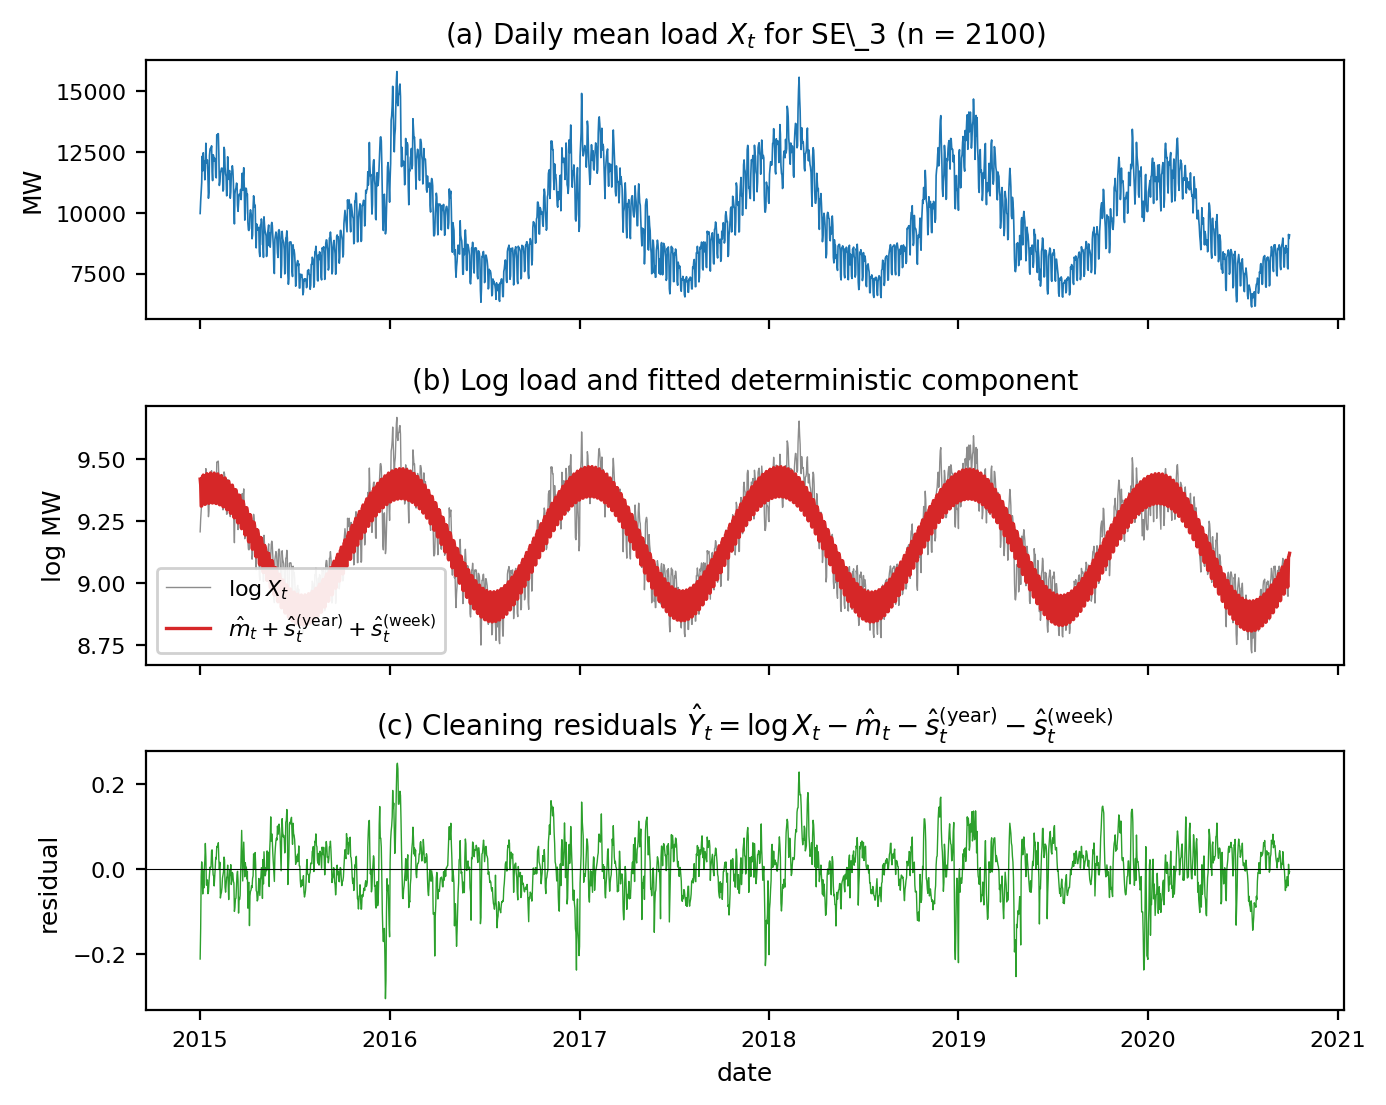
\includegraphics[width=0.72\linewidth]{figures/fig_decomposition.png}
\caption{Classical decomposition (B\&D~\S1.5) of daily SE\_3 load,
2015-01-01 to 2020-09-30. (a)~Raw daily mean load $X_t$, $n = 2100$.
(b)~Log-load $\log X_t$ (grey) overlaid with the fitted deterministic component
$\hat m_t + \hat s_t^{(\mathrm{year})} + \hat s_t^{(\mathrm{week})}$ (red);
seasonals are harmonic regressions ($d=365, k=2$ and $d=7, k=3$) and the trend
is a quadratic OLS fit. (c)~Cleaning residuals $\hat Y_t$ entering the ARMA stage.}
\label{fig:decomposition}
\end{figure}

\begin{figure}[H]
\centering
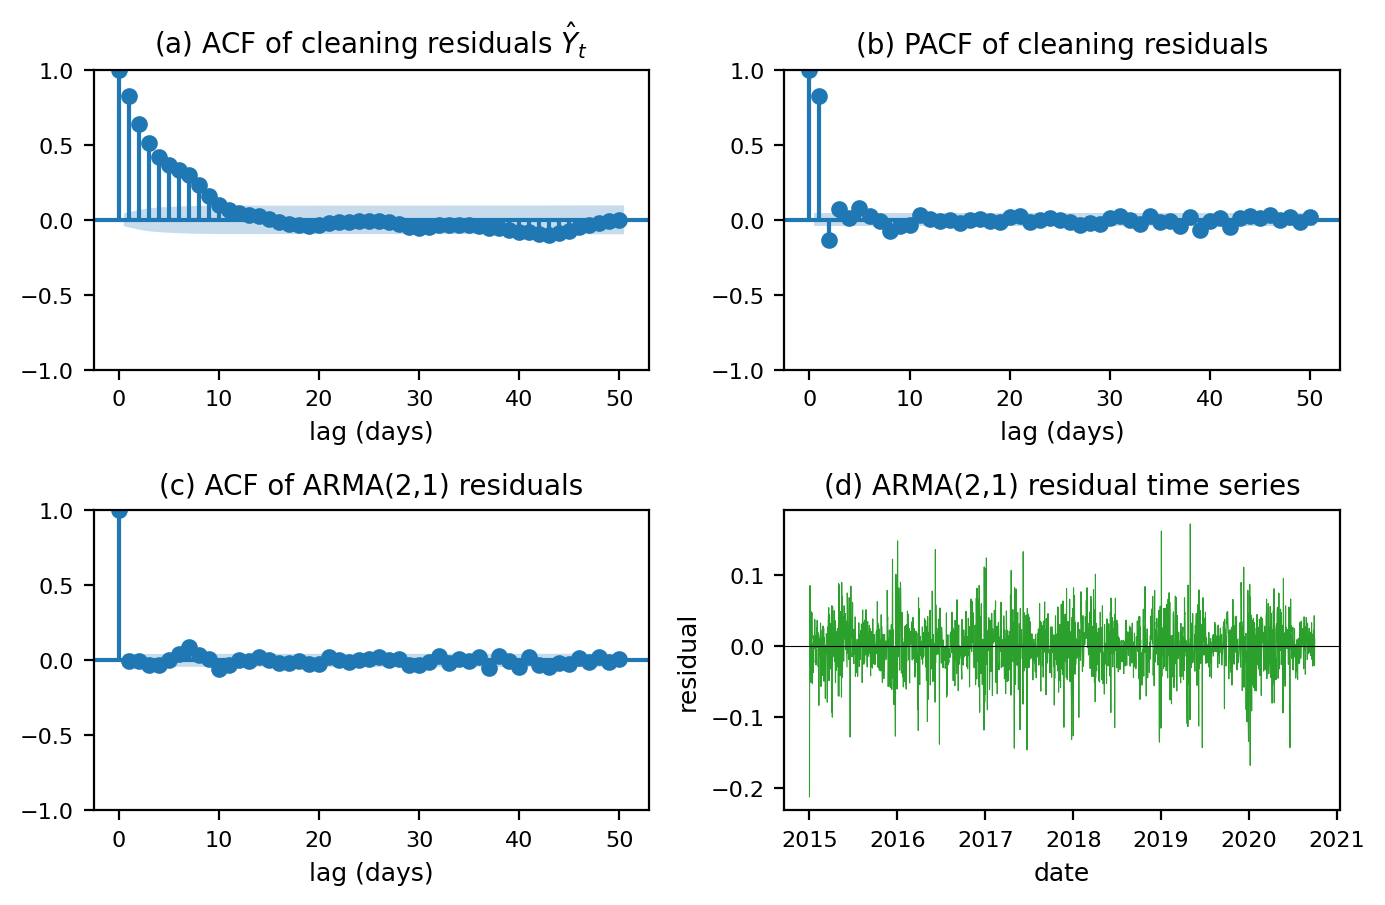
\includegraphics[width=0.78\linewidth]{figures/fig_diagnostics.png}
\caption{Diagnostic plots. (a)~Sample ACF of cleaning residuals $\hat Y_t$
(lags 0--50, blue bands at $\pm 1.96/\sqrt{n}$, B\&D~\S1.4.1). Slow decay
$\hat\rho(1) = 0.83$ and the lag-7 spike $\hat\rho(7) = 0.30$ motivate an
AR-dominated ARMA fit. (b)~Sample PACF of $\hat Y_t$, largest spike at lag~1.
(c)~ACF of ARMA(2,1) residuals; the surviving correlation is concentrated at
multiples of~7 ($Q(20) = 43.7$, df $=17$, $p = 4\!\times\!10^{-4}$).
(d)~ARMA(2,1) residual time series; level and amplitude stable.}
\label{fig:diag}
\end{figure}

\begin{figure}[H]
\centering
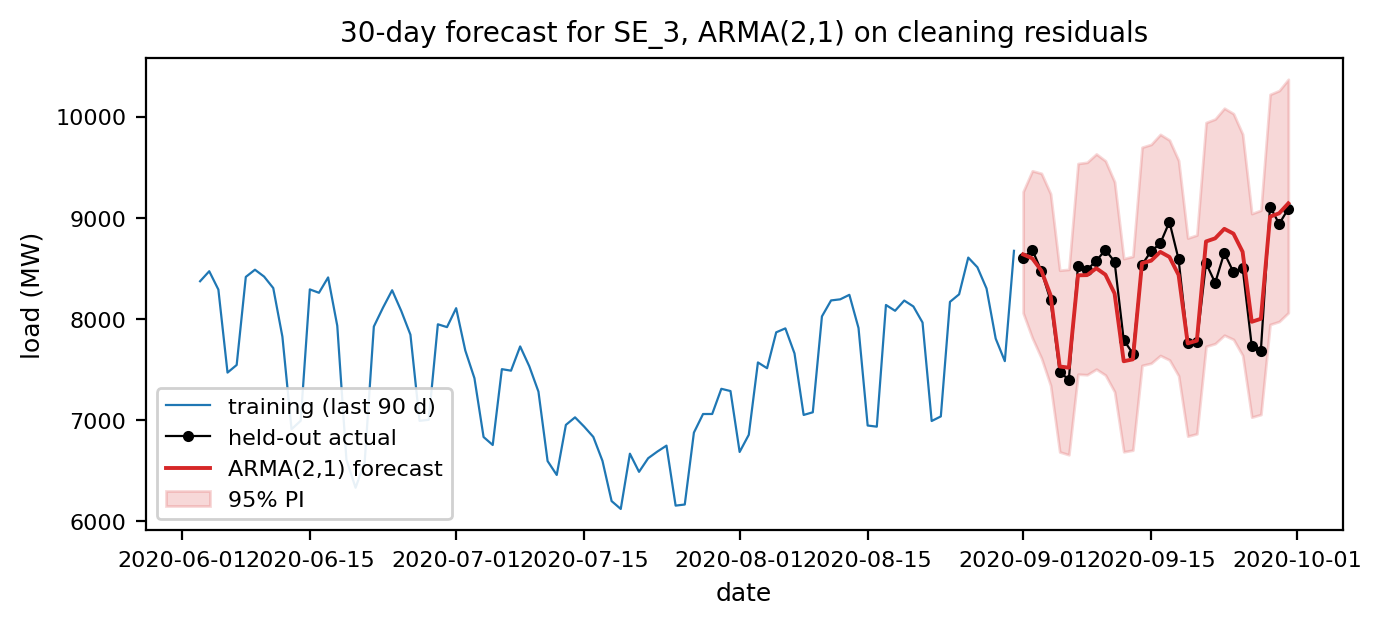
\includegraphics[width=0.88\linewidth]{figures/fig_forecast.png}
\caption{30-day forecast on the held-out window 2020-09-01 to 2020-09-30,
ARMA(2,1) refit on the first $n - 30$ cleaning residuals. Blue: last 90~days
of training. Black markers: held-out actual daily means.
Red: $h$-step ARMA forecast (B\&D~\S3.3.1) inverted to MW by adding the
extrapolated trend and seasonals and exponentiating; red band is the 95\% PI
(log-normal in MW). RMSE $= 187.6$\,MW, MAE $= 145.1$\,MW, empirical PI
coverage $30/30$.}
\label{fig:forecast}
\end{figure}

\end{document}
